
%==============================================
%           Appendix
%==============================================

\newpage
\section{Appendix}

\subsection{Code repositories}
\hspace{0.6cm}

The developed software (and some technical documentation) can be found in a Bitbucket repository linked below.
\newline

\noindent\fcolorbox{logocolor}{white}{%
    \parbox{\textwidth}{%
        \centering
        \href{https://bitbucket.org/3sztof/lhcb_online/src/master/}{The author's open-source code repository (LINK)}. 
    }%
}

\vspace{0.6cm}

\noindent
In the future, the project will be maintained by the main supervisor - Markus Frank. The official, production repository can be found here:
\newline

\noindent\fcolorbox{logocolor}{white}{%
    \parbox{\textwidth}{%
        \centering
        \href{https://gitlab.cern.ch/lhcb/OnlineExtra/tree/master/Online/TaskDB}{The project maintained by Markus Frank in LHCb Gitlab repository (LINK)}. 
    }%
}
\vspace{0.6cm}


%==============================================

\subsection{Database}
\hspace{0.6cm}

A schema of the database tables and their columns recreating the task $\xleftrightarrow{}$ task set $\xleftrightarrow{}$ node class $\xleftrightarrow{}$ node hierarchy is shown in figure \ref{fig:schema}.
\newline

\begin{figure}[H]
\centering
    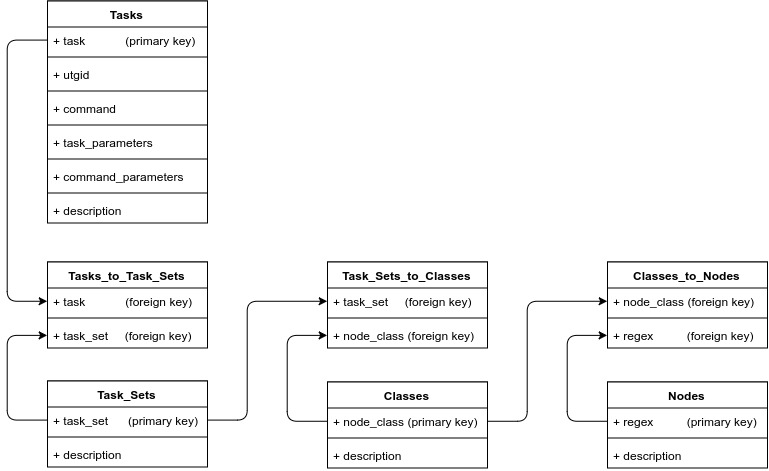
\includegraphics[scale=0.58]{images/Database_Schema.jpg}
    \caption{Database schema diagram}
    \label{fig:schema}
\end{figure}

\newpage
\noindent
To maintain the relationships between the "parent" and "child" data in the hierarchy, it was required to introduce the following three additional tables:

\begin{multicols}{3}
    \begin{itemize}
        \item Tasks\_to\_Task\_Sets
        \item Task\_Sets\_to\_Classes
        \item Classes\_to\_Nodes
    \end{itemize}
\end{multicols}

\noindent
Those three structures contain pairs of assignments that allow the creation of "many to many" relationships between the primary keys (unique names) of the assigned items and their parent tables. For example, one task can belong to many tasks sets while one task set can contain many tasks. 
\newline

%==============================================

\noindent
The arrows visible on figure \ref{fig:schema} were meant to visualize the constraints that were put on the data entries. Besides the "unique" primary keys, the database utilizes "foreign key" mechanism that was needed to introduce many to many relationship between the tables of sets and items assigned to the sets. 
\newline

\noindent
The behaviour of data referenced to as a "foreign key" has to be defined in case the primary key it references is deleted or updated. In the current solution, two events were defined:

\begin{itemize}
    \item On update cascade \\ (update the foreign key if the original value was updated in its mother table)
    \item On delete cascade \\ (delete the foreign key if the original value was deleted from its mother table)
\end{itemize}

%==============================================

\noindent
The database engine used in the current solution is SQLite as it is an integral part of both Python 2.7 and Python 3 - this way no maintaining is needed after software upgrade, the dependencies should be kept safe.
\newline

\noindent
While most of the early python scripts used sqlite3 Python module to connect to the database, the final Main API script utilizes sqlalchemy (foreign module) as it allows for easier transition to other database engines (relational) should the situation demand it in the future. Sqlalchemy connection and query objects are compatible with the database engines such as SQLite, Postgresql, MySQL, Oracle, MS-SQL, Firebird, Sybase and many others.

%==============================================

\subsection{Main API methods}
\hspace{0.6cm}

The Main API methods were implemented as methods of a Python class named "TaskDB". The following points contain their brief descriptions and sample method calls. Note that the parameters of the example calls put in angle brackets, like "<key>" are mandatory and specifying their key name is optional (they can be passed just as a value in the correct order), the others are optional.  


\newpage
\begin{itemize}
    % Add
    \item 
        \textbf{addItem} (where "Item" should be replaced with "Task", "TaskSet", "Class" or "Node"): creates a new entry in the specified Item's table. The required value is the table's primary key (see figure \ref{fig:schema}). Note that specifying only the primary key is not enough for a Task configuration to be considered complete: in order for it to work correctly, at least "utgid" and "command" values (required by pcAdd) should also be specified.

        \begin{sexylisting}[colback=white]{addItem method call}
TaskDB.addTask(<task>="SampleTask",
               utgid="UserDefinedIdentifier",
               command="sleep.sh",
               command_parameters="-t 3",
               description="Sleep for 3 seconds")
        \end{sexylisting}
    
    % Delete
    \item 
        \textbf{deleteItem} (where "Item" should be replaced with "Task", "TaskSet", "Class" or "Node"): deletes an entry from the specified Item's table. The only (and required) parameter of this method is Item's primary key (unique name). Note that when deleting an entry this way, all of its foreign key dependencies will also be deleted.
        
        \begin{sexylisting}[colback=white]{deleteItem method call}
TaskDB.deleteTask(<task>="SampleTask")
        \end{sexylisting}
    
    % Modify
    \item 
        \textbf{modifyItem} (where "Item" should be replaced with "Task", "TaskSet", "Class" or "Node"): modifies the specified Item's data when given correct keys and values, or leaves them unchanged otherwise.
        \begin{sexylisting}[colback=white]{modifyItem method call}
TaskDB.modifyTask(<original_task>="SampleTask",
                  task="ModifiedTask", 
                  description="This task was modified")
        \end{sexylisting}
    
    % Get
    \item 
        \textbf{getItem} (where "Item" should be replaced with "Task", "TaskSet", "Class" or "Node"): returns a JSON object containing all of the Item's data (in "data" root value array). If no argument is specified, or "*" is provided, the method will return (by default) all of the Items of given type.
        \begin{sexylisting}[colback=white]{getItem method call}
TaskDB.getTask(<task>="SampleTask")
        \end{sexylisting}
        \begin{sexylisting}[colback=white]{getItem response}
{"data":[
    {
        "task": "SampleTask",
        "description": "Sample task's description
    }
]}
        \end{sexylisting}
    
    % Assign
    \item 
        \textbf{assignItem} (where "Item" should be replaced with "Task", "TaskSet" or "Class"): assigns the specified Item to its parent. Two parameters are required: one pointing to the primary key of the child (item to be assigned) and the other pointing to the primary key of an existing set.
        \begin{sexylisting}[colback=white]{assignItem method call}
TaskDB.assignTask(<task>="SampleTask", 
                  <task_set>="SampleTaskSet")
        \end{sexylisting}
        \begin{sexylisting}[colback=white]{assignItem method call}
TaskDB.assignClass(<node_class>="SampleNodeClass", 
                   <regex>="SampleNodeRegex")
        \end{sexylisting}
        
    % Unassign
    \item 
        \textbf{unassignItem} (where "Item" should be replaced with "Task", "TaskSet" or "Class"): unassigns the specified Item from its parent. Two parameters are required: one pointing to the primary key of the child (item to be unassigned) and the other pointing to the primary key of an existing set.
        \begin{sexylisting}[colback=white]{unassignItem method call}
TaskDB.unassignTask(<task>="SampleTask", 
                    <task_set>="SampleTaskSet")
        \end{sexylisting}
        \begin{sexylisting}[colback=white]{unassignItem method call}
TaskDB.unassignClass(<node_class>="SampleNodeClass", 
                     <regex>="SampleNodeRegex")
        \end{sexylisting}
      
\newpage  
    % InSet
    \item
        \textbf{itemsInSet} (where "items" should be replaced with "tasks", "tasksets" or "nodeclass" and "Set" should be replaced with "Set", "Class" or "Node" accordingly): returns a JSON object containing all of the items assigned to a given set. The only required parameter is the Set's primary key (unique name).
        \begin{sexylisting}[colback=white]{itemsInSet method call}
TaskDB.tasksetsInClass(<node_class>="SampleNodeClass")
        \end{sexylisting}
        \begin{sexylisting}[colback=white]{itemsInSet response}
{"data":[
    {
        "task_set": "SampleTaskSet",
    },
    {
        "task_set": "AnotherSampleTaskSet"
    }
]}
        \end{sexylisting}
        
    % GetTasksByNode
    \item
        \textbf{getTasksByNode}: returns all of the tasks that should be started on a specified node (regular expression) in a form of an array. If "*" is provided as an argument, the method will return all of the tasks that are assigned to all of the existing nodes.
        \begin{sexylisting}[colback=white]{getTasksByNode method call}
TaskDB.getTasksByNode(<node>="*")
        \end{sexylisting}
        
        % Edit the above (update after changes in the API)
        
\end{itemize}


%Something about other Classes in the script? Connection?


%==============================================

\subsection{Front-end connectors}
\hspace{0.6cm}

In the latest version of the system, both JSONRPC and XMLRPC protocols can be used to interact with the Main API using the POST HTTP method and JSON/XML request body. The following call and response examples aim to show a similarity between the two protocols and deepen the reader's understanding of what is happening in the back-end $\xleftrightarrow{}$ front-end communication layer.

\newpage
\begin{itemize}
    \item 
        JSONRPC
        \begin{sexylisting}[colback=white]{JSONRPC request body}
{
    "jsonrpc": "2.0", 
    "method": "getSet", 
    "params": {"task_set": "SampleSet"}, 
    "id": 3
}
        \end{sexylisting}
        \begin{sexylisting}[colback=white]{JSONRPC response body}
{
    "jsonrpc": "2.0",
    "result":
        [
            {
                "task_set": "SampleSet", 
                "description": "Description"
            }       
        ],
    "id": 3
}
        \end{sexylisting}
    \item
        XMLRPC
        \begin{sexylisting}[colback=white]{XMLRPC request body}
<?xml version='1.0'?> 
<methodCall>
    <methodName>getSet</methodName>\n 
    <params>
    <param>
        <value><struct>
        <member>
            <name>task_set</name>
            <value><string>SampleSet</string></value>
        </member>
        </struct></value>
    </param>
    </params>
</methodCall>
        \end{sexylisting}
        \begin{sexylisting}[colback=white]{XMLRPC response body}
<?xml version='1.0'?>
<methodResponse>
    <params>
    <param>
        <value><array><data>
        <value><struct>
        <member>
            <name>task_set</name>
            <value><string>SampleSet</string></value>
        </member>
        <member>
            <name>description</name>
            <value><string>Description</string></value>
        </member>
        </struct></value>
        </data></array></value>
    </param>
    </params>
</methodResponse>
        \end{sexylisting}
\end{itemize}

\noindent
The links below point to the specifications of JSONRPC and XMLRPC protocols, should the reader be interested in more advanced features.
\newline

\noindent\fcolorbox{logocolor}{white}{%
    \parbox{\textwidth}{%
        \centering
        \href{https://www.jsonrpc.org/specification}{JSONRPC protocol specification (LINK)}. 
    }%
}
\newline

\noindent\fcolorbox{logocolor}{white}{%
    \parbox{\textwidth}{%
        \centering
        \href{http://xmlrpc.scripting.com/spec.html}{XMLRPC protocol specification (LINK)}. 
    }%
}

%==============================================

%\subsection{Command line interface}
%\hspace{0.6cm}

%aa

%==============================================

\subsection{Sencha CMD tool}
\hspace{0.6cm}

The Sencha Ext JS application (graphical front-end) was submitted to the repository in a minimized form - the complete build directory contained over 25000 automatically generated files and was taking over 370 MB of disk space. All of those dependencies are only required to run the debugging and the development server, most of them were belonging to Ext JS SDK (GPL, version 6.2.0).
\newline

\noindent
While the full structure of the development folder is not needed for simple deployment of the application, it might be required to fix some bugs or extend its functionality in the future. For this, one needs to regenerate the development environment using Sencha CMD tool.

\newpage
\noindent
The tools needed for environment regeneration are:
\newline

\noindent\fcolorbox{logocolor}{white}{%
\parbox{\textwidth}{%
    \centering
    \href{https://www.sencha.com/products/extjs/cmd-download/}{Sencha CMD tool (LINK) \\ (v6.6.0.13 has been used during the application development)}  
    }%
}
\vspace{0.3cm}

\noindent\fcolorbox{logocolor}{white}{%
\parbox{\textwidth}{%
    \centering
    \href{https://www.sencha.com/legal/gpl/}{Sencha Ext JS SDK, GPL (LINK) \\ (v6.2.0 has been used during the application development)}  
    }%
}
\newline

\noindent
To build the application from the source, the following actions are needed:

\begin{itemize}
    \item
        Modify the workspace.json file to specify path to the Sencha Ext JS SDK directory. The version is an optional parameter that should be changed in case of SDK version upgrade. The workspace.json file fragment indicating this path should look like this:
        \begin{sexylisting}[colback=white]{workspace.json for fast building}
"frameworks": {
    "ext": {
        "path":"/home/einstein/ext-6.2.0",
        "version":"6.2.0.981"
    }
}
        \end{sexylisting}
        
    \item
        Generate a sample Ext JS application to recreate the build environment by running the command provided in the following code example outside the application's root folder:
        \begin{sexylisting}[colback=white]{environment regeneration}
>mkdir temp
>sencha -sdk /home/einstein/ext-6.2.0 generate app
 MyApp temp
        \end{sexylisting}
        Then, recursively copy (cp -r) the hidden ".sencha/" directory from the sample application's directory (temp) to the root directory of the original project.
        
    \item
        In the application's root directory, run the command provided in the next code example to build the application in "./build/<type>/LHCb".
        \begin{sexylisting}[colback=white]{application building}
>sencha app build (defaults to production build)
>sencha app build testing (more logging in JS console)
        \end{sexylisting}
\end{itemize}

\noindent
The application built this way should be ready to be deployed on an Apache server with proxy routing to the back-end services on the same port (or the development file/service server provided in the TaskDB folder).

\noindent
To run the application in exhaustively debugging mode (a server provided by Sencha CMD tool, on port 1841, which constantly updates the hosted file system - continuous building), one needs to take the following steps:

\begin{itemize}
    \item
         Modify the workspace.json file to specify path to a minimized SDK copy in the application's root directory. The version is an optional parameter that should be changed in case of SDK version upgrade. The workspace.json file fragment indicating this path should look exactly like this:
        \begin{sexylisting}[colback=white]{workspace.json for debug building}
"frameworks": {
    "ext": {
        "path":"ext",
        "version":"6.2.0.981"
    }
}
        \end{sexylisting}
    \item
        Generate a sample Ext JS application to recreate the build environment by running the command provided in the following code example outside the application's root folder:
        \begin{sexylisting}[colback=white]{environment regeneration}
>mkdir temp
>sencha -sdk /home/einstein/ext-6.2.0 generate app
 MyApp temp
        \end{sexylisting}
        Then, recursively copy (cp -r) the hidden ".sencha/" and "ext/" directories from the sample application's directory (temp) to the root directory of the original project.
    \item
        In the application's root directory, run the command provided in the next code example to deploy the debugging server on local port 1841.
        \begin{sexylisting}[colback=white]{starting the debug server}
>sencha app watch
        \end{sexylisting}
\end{itemize}

\newpage

\noindent
The Sencha CMD tool can also be used to upgrade the application to newer versions of Ext JS SDK (GPL) should the situation demand it in the future. This can be achieved by simply running the command provided in the next code example in the application's root directory.

\begin{sexylisting}[colback=white]{starting the debug server}
>sencha app upgrade [path to updated framework]
\end{sexylisting}

\noindent
Please be warned that this operation might require further changes if customization has been applied to the automatically generated files. For more details on the upgrade function of Sencha CMD tool, consult the guide linked below.
\newline

\noindent
\fcolorbox{logocolor}{white}{%
\parbox{\textwidth}{%
    \centering
    \href{https://docs.sencha.com/cmd/guides/cmd_upgrade.html}{Sencha CMD tool upgrade operation (LINK)}  
    }%
}
